%! Author = joels
%! Date = 27/01/2022

\section{Lexikanische Analyse}
\textbf{$\rightarrow$ Kümmert sich um die lexikanische Analyse}\\
\textbf{Input:} Zeichenfolge (Programmtext)\\
\textbf{Output:} Folge von Terminalsymbolen (Tokens)\\
\textbf{Aufgaben:}
\begin{itemize}[topsep=0pt]
    \itemsep -0.2em
    \item Fasst Textzeichen zu Tokens zusammen
    \item Eliminiert Whitespaces und Kommentare
    \item Merkt Position in Programmcode für Fehlermeldung/Debugging
\end{itemize}
\textbf{Nutzen:}\\
$\rightarrow$ Erleichtert spätere syntaktische Analyse (Parser)
\begin{itemize}[topsep=0pt]
    \itemsep -0.2em
    \item Abstraktion: Parser muss sich nicht um Textzeichen kümmern
    \item Einfachheit: Parser braucht Lookahead pro Symbol, nicht Textzeichen
    \item Effizienz: Lexer benötigt Stack im Gegensatz zu Parser
\end{itemize}
\subsection{Tokens}
\begin{itemize}[topsep=0pt]
    \itemsep -0.2em
    \item \textbf{Statisch:} Keywords, Operationen, Interpunktion
    \SubItem{if, else, while, *, \&\&, ;}
    \item \textbf{Identifiers}
    \SubItem{MyClass, readFile, name2}
    \item \textbf{Zahlen}
    \SubItem{123, oxfe12, 1.2e-3}
    \item \textbf{Strings}
    \SubItem{\dq Hello!\dq, \dq \dq, \dq 01234\dq, \dq $\backslash$n\dq}
    \item \textbf{Evt weitere}
    \SubItem{Einzelne Characters wie 'a', '0'}
\end{itemize}

\subsection{Reguläre Sprachen}
\textbf{Regulär: Als EBNF ohne Rekursion ausdrückbar!!}\\
\linebreak
\begin{minipage}{0,5\linewidth}
    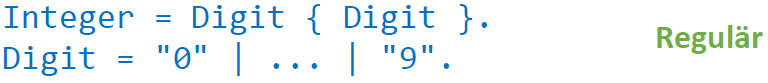
\includegraphics[width=\linewidth]{regulaere_sprachen_1}\\
    
\includegraphics[width=\linewidth]{regulaere_sprachen_2}\\
    \linebreak
    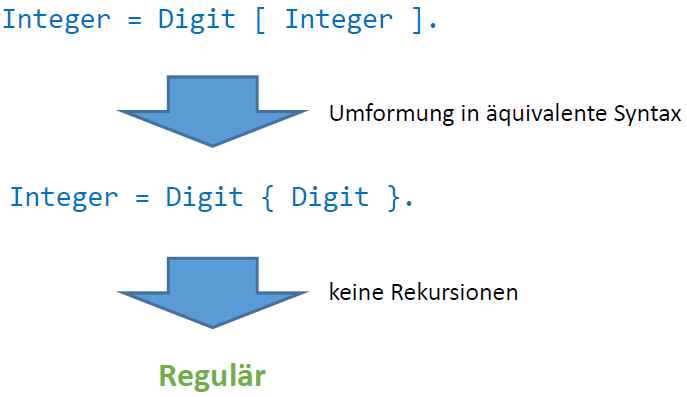
\includegraphics[width=\linewidth]{regulaere_sprachen_3}
\end{minipage}
\begin{minipage}{0,5\linewidth}
    \textbf{Chomsky Hierarchie}\\
    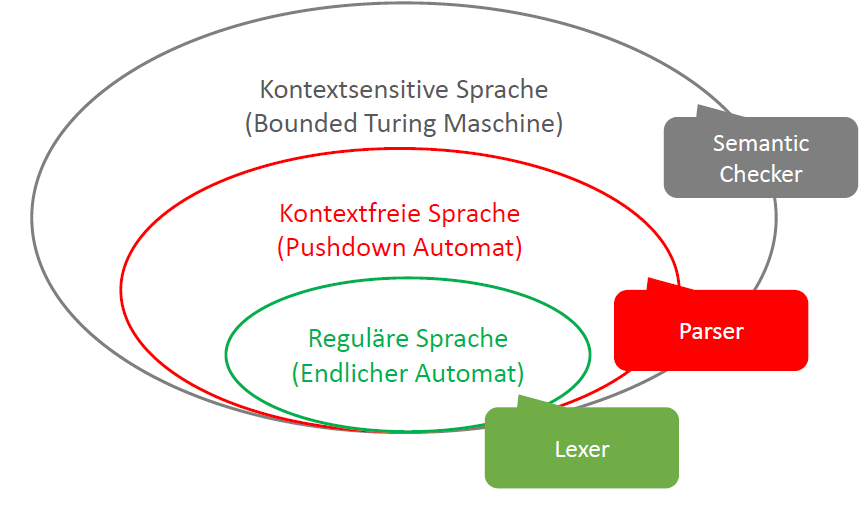
\includegraphics[width=\linewidth]{chomsky_hierarchie}
\end{minipage}
\subsection{Identifier}
\begin{minipage}{0,4\linewidth}
    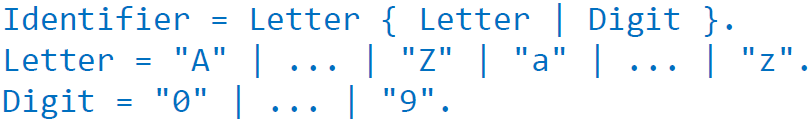
\includegraphics[width=\linewidth]{identifier}
\end{minipage}
\begin{minipage}{0,6\linewidth}
    \begin{itemize}[topsep=0pt]
        \itemsep -0.2em
        \item Bezeichner von Klassen Methoden, Variablen etc.
        \item Beginnt mit Buchstabe, danach Ziffern erlaubt
        \item (Java unterstützt auch Underscores, wir nicht)
    \end{itemize}
\end{minipage}
\subsection{Sonstiges}
\begin{itemize}[topsep=0pt]
    \itemsep -0.2em
    \item \textbf{Maximum Munch:} Lexer absorbiert möglichst viel in einem Token
    \item \textbf{Whitespaces:} Von Lexer übersprungen, trennt Tokens, Tokens evt auch ohne Whitespac getrennt
    \item \textbf{Von Lexer übersprungen}
    \SubItem{Blockkommentare: Nicht schachtelbar, weil sonst nicht mehr regulär}
    \SubItem{Zeilenkommentar:} Bis Newline
\end{itemize}
\subsection{Token-Model}
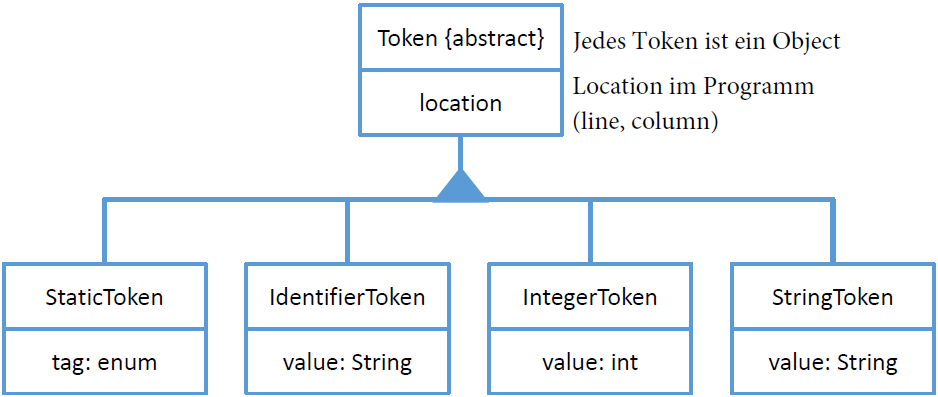
\includegraphics[width=0.7\linewidth]{token_model}

\subsection{Implementation}
\subsubsection{Tags für statische Tokens}
Tipp: Reservierte Typnamen (void, boolean, int, string) und Werte (null, true, false) als Identifier im Lexer verarbeiten.
\begin{lstlisting}
public enum Tag {
    CLASS,ELSE ,IF ,RETURN ,WHILE, ...
    AND, OR, PLUS, MINUS, SEMICOLON, ...
}
\end{lstlisting}

\subsubsection{Lexer Gerüst}
\begin{lstlisting}
class Lexer {
    private final Reader reader;
    private char current; // One character lookahead
    private boolean end;

    private Lexer(Reader reader) {
        this.reader = reader;
    }

    public static Iterable<Token> scan(Reader reader) {
        return new Lexer(reader).readTokenStream();
    }
}
\end{lstlisting}

\subsubsection{Token Stream lesen}
\begin{lstlisting}
Iterable<Token> readTokenStream() {
    var stream = new ArrayList<Token>();
    readNext(); // Initialisierung: One Character Lookahead
    skipBlanks(); // Whitespaces vor Token eliminieren
    while(!end) {
        stream.add(readToken()); // Nächstes Token
        skipBlanks(); // Whitespaces nach Token eliminieren
    }
    return stream;
}
\end{lstlisting}

\subsubsection{Lexer Kernlogik}
\begin{lstlisting}
Token readToken() {
    if (isDigit(current)) {
        return readInteger();
    }
    if (isLetter(current)) {
        return readName();
    }
    return switch(current) {
        case '"': readString();
        case '+': readStaticToken(Tag.Plus);
        case '-': readStaticToken(Tag.Minus);
        ...
    }
}
\end{lstlisting}